% Created 2016-05-09 Mon 12:19
\documentclass[11pt, a4paper]{article}
\usepackage[utf8]{inputenc}
\usepackage[T1]{fontenc}
\usepackage{fixltx2e}
\usepackage{graphicx}
\usepackage{longtable}
\usepackage{float}
\usepackage{wrapfig}
\usepackage{soul}
\usepackage{textcomp}
\usepackage{marvosym}
\usepackage{wasysym}
\usepackage{latexsym}
\usepackage{amssymb}
\usepackage{hyperref}
\tolerance=1000
\usepackage{minted}
\usepackage[utf8]{inputenc}
\usepackage[english]{babel}
\usepackage{graphicx}
\usepackage[left=2.35cm, right=3.35cm, top=3.35cm, bottom=3.0cm]{geometry}
\usepackage{titling}
\providecommand{\alert}[1]{\textbf{#1}}

\title{Statistical methods for bioinformatics \linebreak Beyond linearity}
\author{Cedric Lood}
\date{\today}
\hypersetup{
  pdfkeywords={},
  pdfsubject={},
  pdfcreator={Emacs Org-mode version 7.9.3f}}

\begin{document}

\maketitle


\graphicspath{ {figures/} }
\setlength{\droptitle}{-5em} 
\setlength{\parindent}{0cm}

\section{Exercise 1}
\label{sec-1}
\subsection{Part a}
\label{sec-1-1}

This is straightforward by taking the coefficients $a_1=\beta_0,
b_1=\beta_1, c_1=\beta_2, d_1=\beta_3$
\subsection{Part b}
\label{sec-1-2}

Since we are looking at $x>\xi$, we have the form:

\begin{itemize}
\item $f(x)=\beta_0 + \beta_1 x + \beta_2 x^2 + \beta_3 x^3 + \beta_4 (x - \xi)^3$
\end{itemize}

We can distribute the cube and get:

\begin{itemize}
\item $f(x)=\beta_0 + \beta_1 x + \beta_2 x^2 + \beta_3 x^3 + \beta_4 (x^3 - 3 x^2 \xi + 3 x \xi^2 - \xi^3)$
\end{itemize}

The expression can be re-arranged to highlight the predictors
coefficients' values:
 
\begin{itemize}
\item $f(x)=(\beta_0 - \beta_4 \xi^3) + (\beta_1 + 3 \beta_4 \xi^2) x +(\beta_2 - 3 \beta_4 \xi) x^2 + (\beta_3 + \beta_4) x^3$
\end{itemize}

Combining with the answer of Part a, we now see that $f(x)$ is a
piecewise polynomial
\subsection{Part c}
\label{sec-1-3}


Showing that the 2 pieces are connected continuously can be done by
solving both in $\xi$:

\begin{itemize}
\item $f_1(\xi)=\beta_0 + \beta_1 \xi + \beta_2 \xi^2 + \beta_3 \xi^3$
\item $f_2(\xi)=(\beta_0 - \beta_4 \xi^3) + (\beta_1 + 3 \beta_4 \xi^2) \xi  +(\beta_2 - 3 \beta_4 \xi) \xi^2 + (\beta_3 + \beta_4) \xi^3$
\end{itemize}

When distributing the terms in $f_2(\xi)$, one obtains that the terms
in $\beta_4$ cancel each other, and that $f_2(\xi)=\beta_0 + \beta_1 \xi + \beta_2 \xi^2 + \beta_3 \xi^3=f_1(\xi)$
\subsection{Part d}
\label{sec-1-4}

For this, we need the first order derivatives of $f_1(x)$ and $f_2(x)$
\begin{itemize}
\item $f_1'(x)=\beta_1 + 2\beta_2 x + 3\beta_3 x^2$
\item $f_2'(x)=\beta_1 + 3 \beta_4 x^2 + 2 (\beta_2 - 3 \beta_4 x) x + 3 (\beta_3 + \beta_4) x^2$
\end{itemize}

Solving the equations above for $x=\xi$:

\begin{itemize}
\item $f_1'(\xi)=\beta_1 + 2\beta_2 \xi + 3\beta_3 \xi^2$
\item $f_2'(\xi) = \beta_1 + 3\beta_4 \xi^2 + 2(\beta_2 - 3\beta_4 \xi) \xi + 3(\beta_3 + \beta_4) \xi^2$
\item $f_2'(\xi) = \beta_1 + 3\beta_4 \xi^2 + 2\beta_2 \xi - 6\beta_4 \xi^2 + 3\beta_3 \xi^2 + 3\beta_4 \xi^2$
\item $f_2'(\xi) = \beta_1 + 2\beta_2 \xi + 3\beta_3 \xi^2 + 3\beta_4 \xi^2 + 3\beta_4 \xi^2 - 6\beta_4 \xi^2$
\item $f_2'(\xi) = \beta_1 + 2\beta_2 \xi + 3\beta_3 \xi^2$
\end{itemize}

Hence, $f_1'(\xi)=\beta_1 + 2\beta_2 \xi + 3\beta_3 \xi^2=f_2'(\xi)$
\subsection{Part e}
\label{sec-1-5}

We can take the second order derivatives of $f_1(x)$ and $f_2(x)$,
and solve in $\xi$ to verify if the transition is continuous:

\begin{itemize}
\item $f_1''(x) = 2\beta_2 + 6\beta_3 x$
\item $f_2''(x) = 2(\beta_2 - 3\beta_4 x) + 6(\beta_3 + \beta_4) x = 2\beta_2 + 6\beta_3 x$
\end{itemize}

Hence, $f_1''(\xi) = 2\beta_2 + 6\beta_3 \xi=f_2''(x)$ \\

Combining this with the previous parts, we have shown that $f(x)$ is
indeed a cubic spline, where the piecewise functions $f_1(x)$ and
$f_2(x)$ are indeed connected, and where the first order and second
order derivatives are smoothly connected.
\section{Exercise 9}
\label{sec-2}

Libraries and dataset used in this exercise:


\begin{minted}[]{R}
library(ggplot2)
library(splines)
library(MASS)
library(boot) # did not work with my version of R
attach(Boston)
\end{minted}
\subsection{Part a}
\label{sec-2-1}


As displayed in the graph below, we obtain a very smooth fit of the
dataset using the simple polynomial of degree 3 fit. Towards dis \~{} 11
and 12, we can suspect that there is overfitting going on, given how
few observations we have in that region, and the fit seemingly getting
increasingly steep in the region. The summary of the fit indicates
that all the coefficients are significant.


\begin{minted}[]{R}
lm.fit = lm(nox ~ poly(dis, 3), data = Boston)
summary(lm.fit)

# creation of a grid of values for prediction
dislim = range(dis)
dis.grid = seq(from = dislim[1], to = dislim[2], by = 0.1)

# prediction & plotting
lm.pred = predict(lm.fit, list(dis = dis.grid))
pdf("parta.pdf")
plot(nox ~ dis, data = Boston, col = "darkgrey",main="Boston nox prediction using dis") 
lines(dis.grid, lm.pred, col = "red", lwd = 2)
dev.off()
\end{minted}


\begin{verbatim}
> summary(lm.fit)

Call:
lm(formula = nox ~ poly(dis, 3), data = Boston)

Residuals:
      Min        1Q    Median        3Q       Max 
-0.121130 -0.040619 -0.009738  0.023385  0.194904 

Coefficients:
               Estimate Std. Error t value Pr(>|t|)    
(Intercept)    0.554695   0.002759 201.021  < 2e-16 ***
poly(dis, 3)1 -2.003096   0.062071 -32.271  < 2e-16 ***
poly(dis, 3)2  0.856330   0.062071  13.796  < 2e-16 ***
poly(dis, 3)3 -0.318049   0.062071  -5.124 4.27e-07 ***
---
Signif. codes:  0 ‘***’ 0.001 ‘**’ 0.01 ‘*’ 0.05 ‘.’ 0.1 ‘ ’ 1

Residual standard error: 0.06207 on 502 degrees of freedom
Multiple R-squared:  0.7148,    Adjusted R-squared:  0.7131 
F-statistic: 419.3 on 3 and 502 DF,  p-value: < 2.2e-16
\end{verbatim}

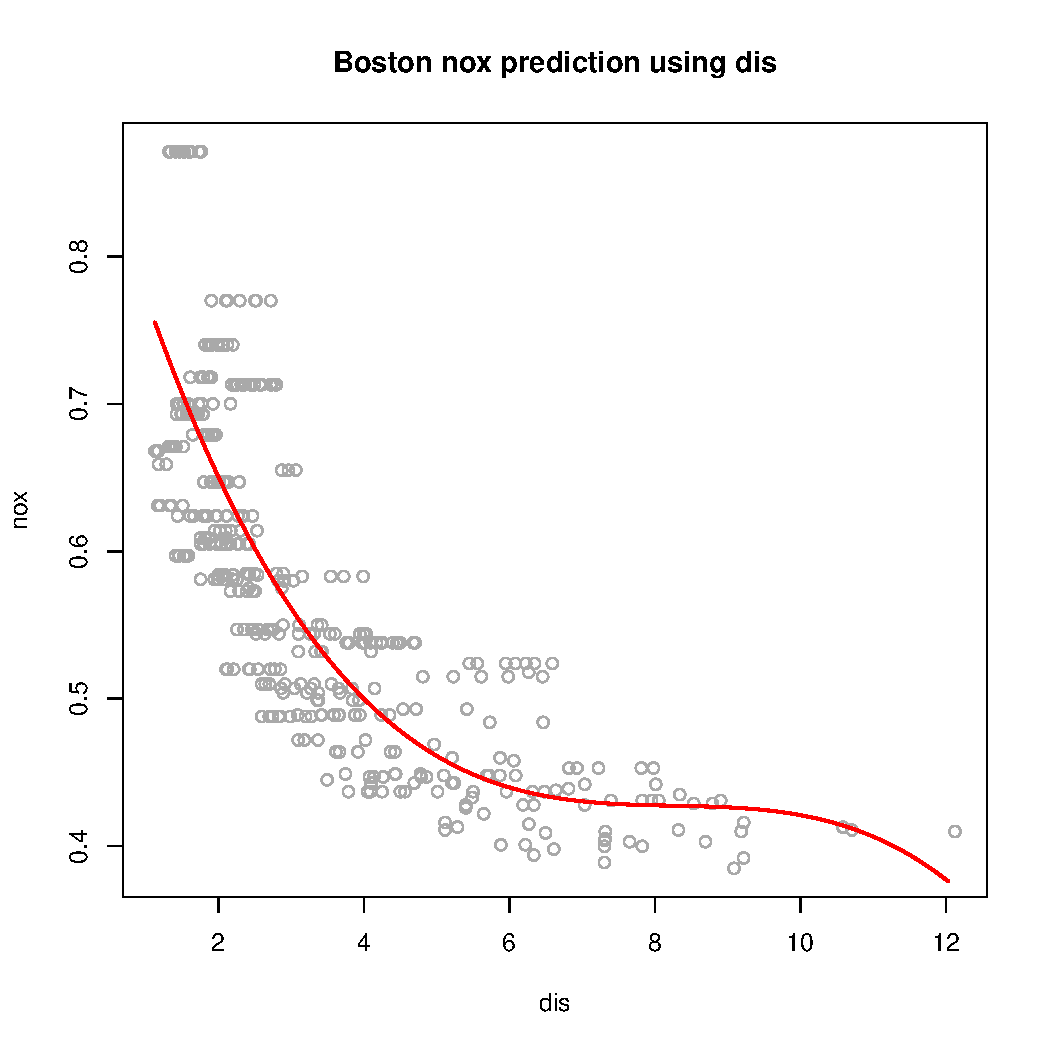
\includegraphics[scale=0.6]{parta.pdf}
\subsection{Part b}
\label{sec-2-2}


As can be expected, the RSS decreases with the degree of the
polynomial (increase in the flexibility of the model). This could be
due to overfitting though, so in the next part we'll investigate the
question using CV.


\begin{minted}[]{R}
all.rss = rep(NA, 10)
for (i in 1:10) {
    lm.fit = lm(nox ~ poly(dis, i), data = Boston)
    all.rss[i] = sum(lm.fit$residuals^2)
}
\end{minted}


\begin{verbatim}
> rss
 [1] 2.768563 2.035262 1.934107 1.932981 1.915290 1.878257 1.849484 1.835630
 [9] 1.833331 1.832171
\end{verbatim}
\subsection{Part c}
\label{sec-2-3}


I would have used the cv.glm function for this section, but the
package boost was not available for my version of R. Instead I used a
simpler validation set approach.

As shown in the graph below, the degrees 3, 6, and 8 are all
contenders to be selected for the model. The error on the validation
set varies widely for degree 7.


\begin{minted}[]{R}
# training using validation set (different seeds)
for (i in 1:10) {
    set.seed(i)
    train <- sample(506,334)
    lm.fit <- lm(nox~poly(dis, i,raw=TRUE), data = Boston, subset=train)
    all.deltas[i] <- mean((nox-predict(lm.fit,Boston))[-train]^2)
}
pdf("partc.pdf")
plot(1:10, all.deltas, xlab = "Polynomial degree", ylab = "Validation set error",
     main="Selection of degree using validation set", type = "l", pch = 20, lwd = 2)
dev.off()
\end{minted}


\begin{verbatim}
> all.deltas
 [1] 0.004923935 0.004082079 0.003632081 0.004410606 0.005002392 0.003807436
 [7] 0.045452142 0.003104770 0.003586399 0.003793285
\end{verbatim}

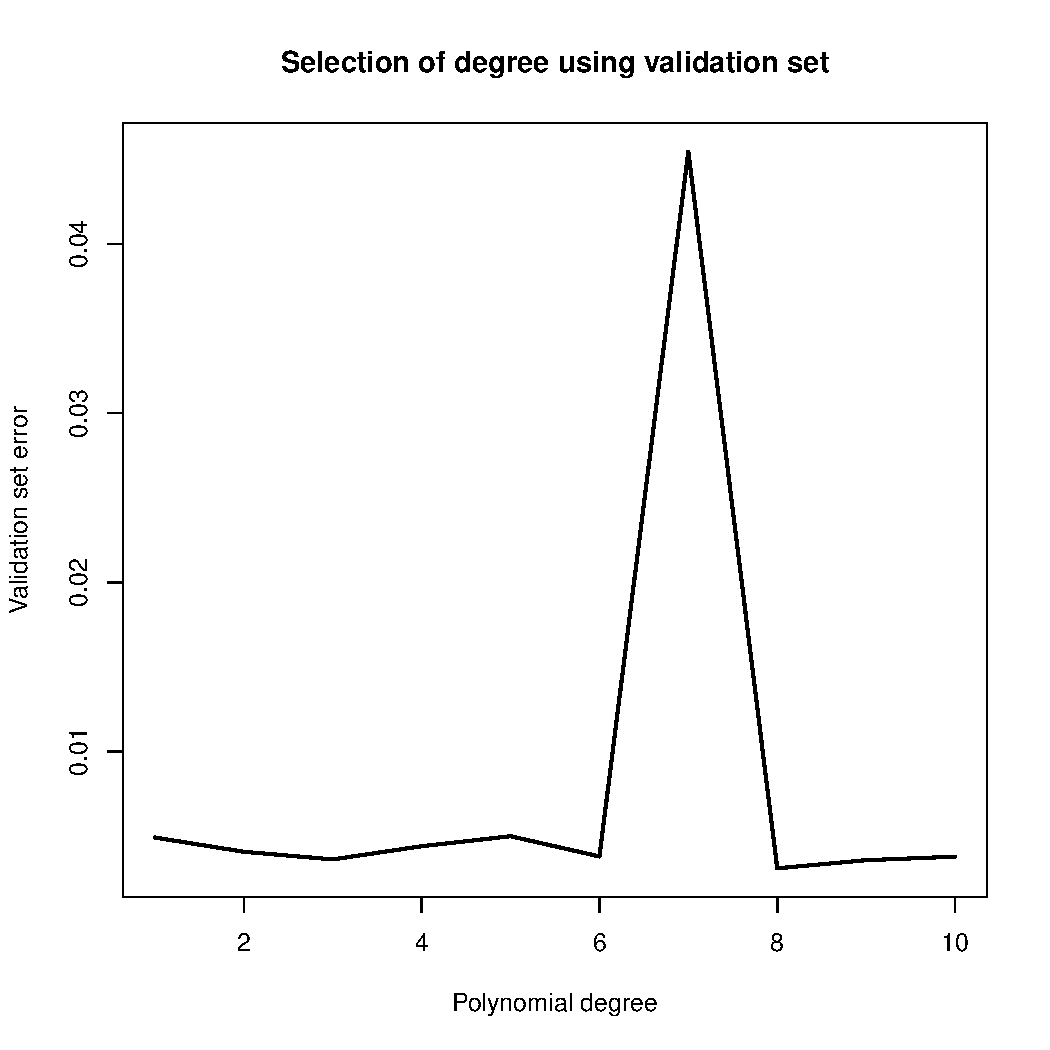
\includegraphics[scale=0.6]{partc.pdf}
\subsection{Part d}
\label{sec-2-4}

As can be observed on the graphic below, the spline seems to fit the
data pretty well. Although the frontier of the dataset (where dis \~{} 11
and 12) displays signs of overfitting with a very ``wobbly'' fit there.

The summary of the fit indicates taht all the coefficients are
significant (see output)


\begin{minted}[]{R}
# range of values for dis, and selection of knots
range(Boston$dis)
k <- c(4,8,11)

# fitting model and plotting results
sp.fit <- lm(nox~bs(dis, df=4, knots=k), data=Boston)
summary(sp.fit)

sp.pred = predict(sp.fit, list(dis = dis.grid))
pdf("partd.pdf")
plot(nox ~ dis, data = Boston, col = "darkgrey", main="Regression spline fit")
lines(dis.grid, sp.pred, col = "red", lwd = 2)
dev.off()
\end{minted}


\begin{verbatim}
> summary(sp.fit)

Call:
lm(formula = nox ~ bs(dis, df = 4, knots = k), data = Boston)

Residuals:
      Min        1Q    Median        3Q       Max 
-0.123651 -0.040031 -0.007984  0.022831  0.193438 

Coefficients:
                            Estimate Std. Error t value Pr(>|t|)    
(Intercept)                  0.74196    0.01314  56.481  < 2e-16 ***
bs(dis, df = 4, knots = k)1 -0.09646    0.02420  -3.985 7.74e-05 ***
bs(dis, df = 4, knots = k)2 -0.34182    0.01824 -18.740  < 2e-16 ***
bs(dis, df = 4, knots = k)3 -0.26067    0.03379  -7.714 6.67e-14 ***
bs(dis, df = 4, knots = k)4 -0.41180    0.04989  -8.254 1.38e-15 ***
bs(dis, df = 4, knots = k)5 -0.21975    0.11785  -1.865   0.0628 .  
bs(dis, df = 4, knots = k)6 -0.33196    0.06332  -5.243 2.34e-07 ***
---
Signif. codes:  0 ‘***’ 0.001 ‘**’ 0.01 ‘*’ 0.05 ‘.’ 0.1 ‘ ’ 1

Residual standard error: 0.06194 on 499 degrees of freedom
Multiple R-squared:  0.7177,    Adjusted R-squared:  0.7143 
F-statistic: 211.4 on 6 and 499 DF,  p-value: < 2.2e-16
\end{verbatim}

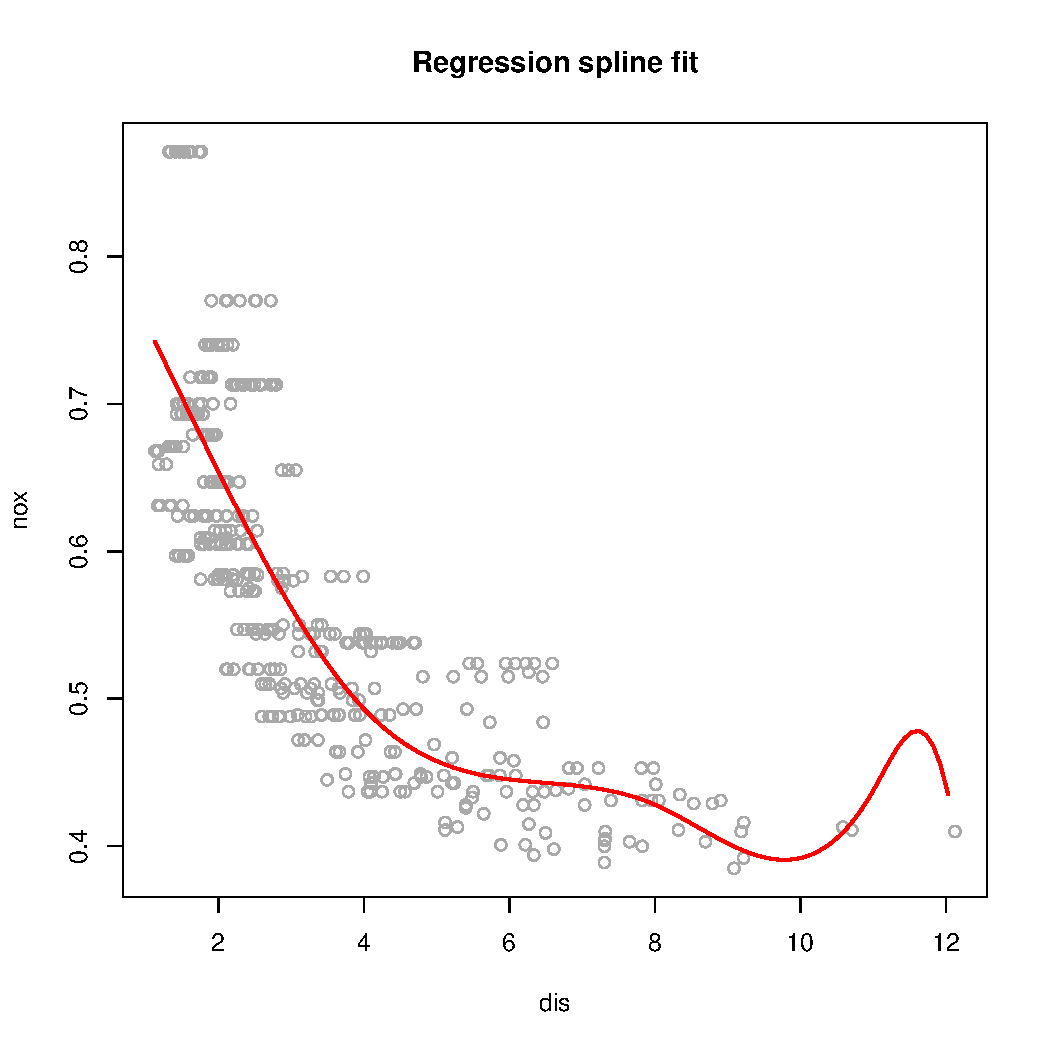
\includegraphics[scale=0.6]{partd.pdf}
\subsection{Part e}
\label{sec-2-5}


Here we observe that the training residuals keep dropping as we add
more degrees of freedom, which is expected. In the next part, we'll
use a validation set to select the correct df.


\begin{minted}[]{R}
all.residuals = rep(NA, 16)

for (i in 3:16) {
    lm.fit = lm(nox ~ bs(dis, df = i), data = Boston)
    all.residuals[i] = sum(lm.fit$residuals^2)
}
all.residuals[-c(1, 2)]
\end{minted}


\begin{verbatim}
> all.residuals[-c(1, 2)]
 [1] 1.934107 1.922775 1.840173 1.833966 1.829884 1.816995 1.825653 1.792535
 [9] 1.796992 1.788999 1.782350 1.781838 1.782798 1.783546
\end{verbatim}
\subsection{Part f}
\label{sec-2-6}


Same remark as in section c concerning the cv.glm function, and the
use of a validation set instead. We can see that the test errors vary
widely with degrees of freedom, although the trend seems to drop
consistently until DF=10.


\begin{minted}[]{R}
all.cv = rep(NA, 16)
set.seed(1)
train <- sample(506,334)
for (i in 3:16) {
    lm.fit = lm(nox ~ bs(dis, df = i), data = Boston,subset=train)
    all.cv[i] <- mean((nox-predict(lm.fit,Boston))[-train]^2)
}

pdf("plotf.pdf")
plot(3:16, all.cv[-c(1, 2)], lwd = 2, type = "l", xlab = "df", ylab = "Validation set error", main="Selection of degrees of freedom")
dev.off()
\end{minted}

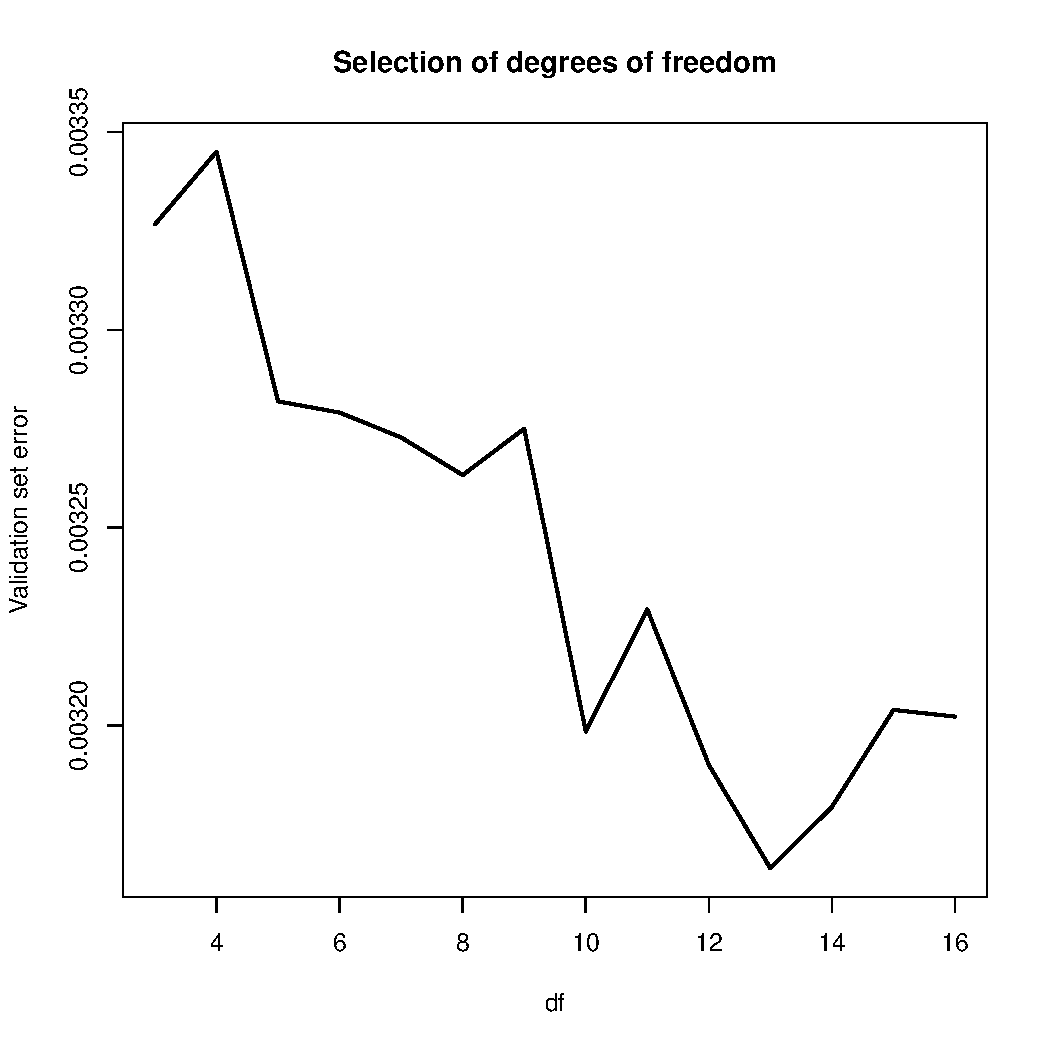
\includegraphics[scale=0.6]{plotf.pdf}

\end{document}
